\chapter{Implementation}
\label{chap:implementation}

Having briefly analysed our approach to the problem, as well as the appropriate decisions we made, we can now proceed to the analysis of the actual implementation of our system.


\section{System Overview}
\label{sec:system-overview}

\begin{figure*}[ht]
\centering
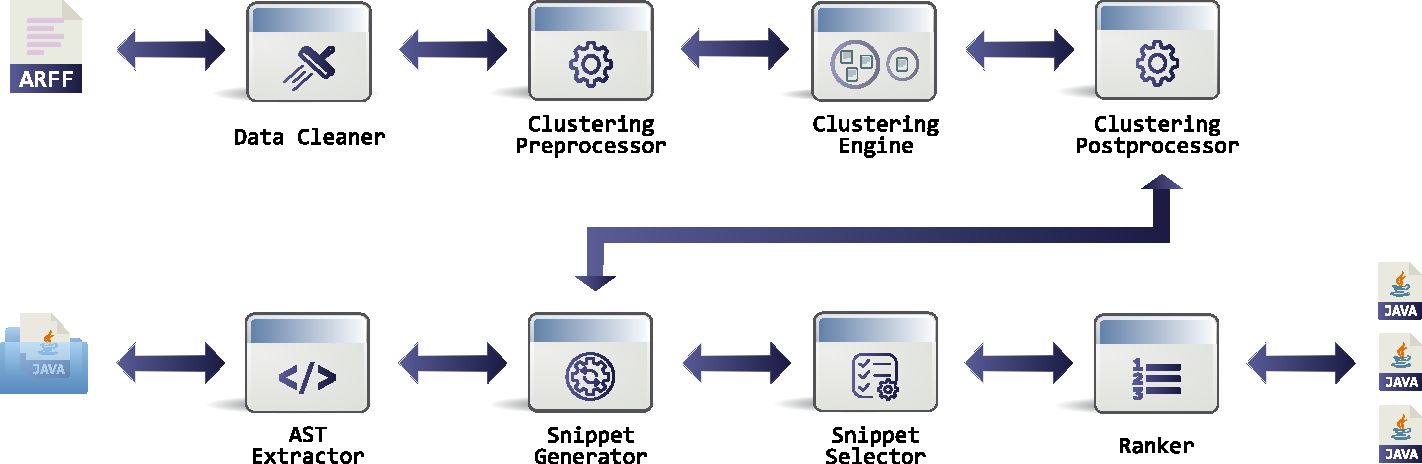
\includegraphics[width=0.9\textwidth]{images/system}
\caption[The architecture of the system]{The architecture of the system.}
\label{images:API-summariser}
\vspace{-2pt}
\end{figure*} 

The architecture of the system is illustrated in \Cref{images:API-summariser}. As depicted, the system comprises the below mentioned components:

\begin{description}
\item[AST Extractor] Extracts the ASTs of the files in the repository.
\item[Data Cleaner] Cleans the \texttt{.arff} file and keeps only the API call sequences that are going to be clustered. 
\item[Clustering Preprocessor] Creates a distance matrix for the sequences, using a sequence distance metric.
\item[Clustering Engine] This is the primary component of the clustering process. It clusters the sequences using the distance matrix and a clustering technique, and stores the results in data structures and files.
\item[Clustering Postprocessor] This component receives the clustering results and identifies the most representative sequences of each cluster. It then retrieves their associated ASTs, which have been extracted by the \text{AST Extractor} component, and feeds them to the \textit{Snippet Generator} component.
\item[Snippet Generator] Generates summarised snippets for the files retrieved by the \textit{Clustering Postprocessor} component, by leveraging the summarisation algorithm.
\item[Snippet Selector] Selects the most representative snippet among the generated snippets of each cluster, based on a tree-edit distance.
\item[Ranker] Ranks the selected snippets based on their support.
\end{description}


\section{AST Extractor}
\label{sec:ast-extractor}

This component extracts the ASTs of the source code files in the repository, which are then used by the \textit{Snippet Generator} component, in order to generate summarised snippets. In order to extract the ASTs, we make use of the \texttt{srcml}\footnote{\url{http://www.srcml.org/about-srcml.html}} tool, which converts Java source code to the \textit{srcML} format. The srcML format is an XML representation for source code, where the mark-up tags identify elements of the abstract syntaxt for the language. An example of the AST extracted by the srcml tool, for a given Java source code, is presented in \Cref{sec:srcml-example}.


\section{Data Cleaner}
\label{sec:data-cleaner}

This component receives the content of the \texttt{.arff} file which, as described in \Cref{sec:input-output}, comprises of client methods and their associated API call sequences, and proceeds to the following modifications, as described in \Cref{sec:data-preprocessing}:

\begin{itemize}
\setlength\itemsep{1pt}
\item Removes callers that refer to different versions of the same source code file.
\item Removes singleton and pseudo-singleton sequences.
\item Removes unique sequences, if specified so by the appropriate parameter.
\end{itemize}

The result of this component is an updated version of the original dataset.

\vspace{-10pt}
\section{Clustering Preprocessor}
\label{sec:clustering-preprocessor}

This component creates a distance matrix, where the distance between any two sequences is stored. The distance metrics that have been implemented in order to compute the distance between any two sequences $S_1$ and $S_2$ are analysed below. Note that both distances are normalised in the range ${[}0.0$,$1.0{]}$.

\vspace{10pt}
\noindent
A. \textit{\underline{LCS distance}}
\vspace{5pt}

This metric makes use of the \textit{Longest Common Subsequence} (LCS) between two sequences, in order to compute their distance. The formula of the \textit{LCS distance} is shown in \Cref{eq:lcs-distance}.
%
\begin{align}
 \label{eq:lcs-distance}
 \centering
  LCS\_dist\left( S_1, S_2 \right) = 
  1 - 2\cdot\frac{ \left| LCS\left( S_1, S_2 \right) \right|}
       {\left| S_1 \right| + \left| S_2 \right|}
\end{align}
%
where $\left|LCS\left( S_1, S_2 \right) \right|$ is the length of the LCS between the two sequences.

As an example, given two sequences $S_1 = BAACD$ and $S_2 = AACBDE$, it holds that $LCS(S_1,S_2) = AACD$, and thus $\left|LCS\left( S_1, S_2 \right) \right| = 4$. Then, the LCS distance is:
%
\begin{align*}
 \centering
  LCS\_dist\left( S_1, S_2 \right) = 
  1 - 2\cdot\frac{ 4}
       {5 + 6} \simeq 0.27
\end{align*}
%
\vspace{10pt}
\noindent
B. \textit{\underline{SeqSim distance}}
\vspace{-2pt}

The \textit{SeqSim} metric is a sequence similarity metric that is based on \textit{n-grams}\footnote{Given a text sequence, an \textit{n-gram} is a contiguous sequence of $n$ items from the given sequence. According to the $n$ value, we may have \textit{unigrams} ($n=1$), \textit{bigrams} ($n=2$) and so on.}, which has been introduced in \cite{Wang:2013}. At first, the authors define the n-gram set $G(S)$, for a sequence $S(s_1s_2 ... s_n)$, as the collection of \textit{unigrams}, \textit{bi-grams}, ... , \textit{n-grams} of $S$, as shown in \Cref{eq:n-grams}:
%
\begin{align}
 \label{eq:n-grams}
  \begin{split}
    G(S) = 
    \lbrace s_1,s_2 ..., s_n,\;\; s_1s_2, s_2s_3 ..., s_{n-1}s_n,\;\; ...,\;\; s_1s_2...s_{n-1}, s_2s_3...s_{n-1}s_n, \\
    s_1s_2...s_{n-1}s_n\rbrace
  \end{split}
\end{align}
%
Then, the distance between $S_1$ and $S_2$ is computed using the formula in \Cref{eq:seqsim}.
%
\begin{equation}
 \label{eq:seqsim}
 \centering
  SeqSim\_dist\left( S_1, S_2 \right) = 
  1 - \frac{ \sum_{i} Weight(g_\cap^{i}) }
       { \sum_{i} Weight(g_\cup^{i}) }
\end{equation}
%
where $G_\cap = G(S_1)\cap G(S_2)$, $G_\cup = G(S_1)\cup G(S_2)$, $g_\cap^{i} \in G_\cap$, $g_\cup^{i} \in G_\cup$, and\\$Weight(g_\cap^{i})$, $Weight(g_\cup^{i})$ are equal to the length of $g_\cap^{i}$ and $g_\cup^{i}$, respectively.


As an example, given two sequences $S_1 = BAACD$ and $S_2 = AACBDE$:
%
\begin{align*}
  G(S_1) &= \lbrace B,A, ..., D,\;\; BA, AA ..., CD,\;\; ...,\;\; BAAC, AACD,\;\; BAACD\rbrace \\
  G(S_2) &= \lbrace A,A, ..., E,\;\; AA, AC ..., DE,\;\; ...,\;\; AACBD, ACBDE,\;\; AACBDE\rbrace \\
  G_\cap &= \lbrace A,B,C,D,\;\; AA,AC,\;\; AAC\rbrace \\
  G_\cup &= \lbrace A,B,...,E,\;\; BA,AA,...DE,\;\;...,BAACD,AACBD,ACBDE,\;\; AACBDE\rbrace
\end{align*}
%
which leads to:
%
\begin{align*}
  SeqSim\_dist\left( S_1, S_2 \right) &= 
  1 - \frac{ Weight(A) + Weight(B) +... + Weight(AAC)}
       { Weight(A) + Weight(B) +... + Weight(AACBDE) } \\
       &= 1 - \frac{ 1 + 1 +... + 3}
       { 1 + 1 +... + 6 } \simeq 0.86
\end{align*}
%
\vspace{15pt}
\noindent
C. \textit{\underline{Jaccard distance}}
\vspace{-10pt}

We have also implemented the \textit{Jaccard} distance. This is basically an itemset distance metric, a fact that makes it not so accurate as the two aforementioned metrics, but it is far more efficient, in terms of computational complexity, and thus it may be used for large datasets. Its formula is presented in \Cref{eq:jaccard}.
%
\vspace{1.5ex}
\begin{equation}
 \label{eq:jaccard}
 \centering
  Jaccard\_dist\left( S_1, S_2 \right) = 
  1 - \frac{ \left| S_1 \cap S_2 \right|}
       {\left| S_1 \cup S_2 \right|}
  \vspace{1.5ex}
\end{equation}
%
As an example, given two sequences $S_1 = BAACD$ and $S_2 = AACBDE$:
%
\vspace{4pt}
\begin{align*}
  Jaccard\_dist\left( S_1, S_2 \right) = 
  1 - \frac{ \left| \lbrace A, B, C, D\rbrace \right|}
       {\left| \lbrace A, B, C, D, E\rbrace \right|} = 1 - \frac{4}{5} = 0.2
  \vspace{15pt}
\end{align*}
%
\Cref{tables:sequence-similarity} shows a few indicative examples that point out the differences between the aforementioned metrics. As we can see, the \textit{Jaccard\_dist} metric may overestimate the similarity between the sequences, while the \textit{SeqSim\_dist} may underestimate it, a fact that could lead to a quite dense or sparse distance matrix respectively. It seems that the \textit{LCS\_metric} provides a balance between the other two metrics. For this reason, we decided to use this metric in the versions of the system that are going to be evaluated.

\begin{table}[ht]
\centering
\small
\caption[Sequence distance metrics examples]{Examples indicating the differences between the various sequence distance metrics that have been implemented.}
\label{tables:sequence-similarity}
\begin{tabular}{lllll}
\toprule
$S_1$ & $S_2$ & $LCS\_dist$ & $SeqSim\_dist$ & $Jaccard\_dist$\\
\midrule
ABC & ABC & 0.00 & 0.0 & 0.00 \\
AB & CDE & 1.00 & 1.00 & 1.00 \\
ACBD & ABDC & 0.25 & 0.82 & 0.00 \\
BAACD & AACBDE & 0.27 & 0.86 & 0.20 \\
AAAB & AAB & 0.14 & 0.44 & 0.00 \\
\bottomrule
\end{tabular}
\end{table}

The outcome of this component is an $N\times N$ table, where $N$ is the number of the sequences. Each sequence is assigned a unique id and, as a result, the value stored in the index $i,j$ of the table is the distance between the $i_{th}$ and the $j_{th}$ sequences\footnote{Although we use a \textit{redundant} (also called \textit{full} or \textit{complete}) distance matrix, we only need the upper triangular part -or even the lower one, as the first one is the transpose of the second one- of the distance matrix, taking into account that this is a symmetric matrix. A more efficient approach would use a \textit{condensed} distance matrix, which does not contain any redundancy.}.


\section{Clustering Engine}
\label{sec:clustering-engine}

The \textit{Clustering Engine} component implements the clustering techniques that could be used in order to cluster the sequences. Although we have integrated/implemented several clustering algorithms, we are going to analyse only the two that are used in the actual implementation. These include an implementation of the $k$-medoids algorithm, as well as the HDBSCAN\footnote{\url{https://github.com/lmcinnes/hdbscan}} algorithm \cite{Campello:2013}.

This component receives the distance matrix as input, and clusters the sequences using one of the implemented clustering techniques, which are analysed in this section.


\subsection{\texorpdfstring{$k$}{k}-medoids Implementation}
\label{subsec:k-medoids-implementation}

The implementation of the $k$-medoids algorithm is based on the one presented in \cite{Bauckhage:2015}. We have also implemented the concept behind the $k$\verb!++! initialisation, in order to predict the initial medoids more efficiently. A simplified pseudocode of the $k$-medoids algorithm that has been implemented is shown in \Cref{algorithms:k-medoids}, while the pseudocode of the $k$\verb!++! initialisation technique is presented in \Cref{algorithms:k++}.

\begin{algorithm}[h]
\small
\caption[$k$-medoids]{$k$-medoids}
\label{algorithms:k-medoids}
\begin{algorithmic}[1]
\Procedure{$k$-medoids}{$k$, $max\_iter$}
    \State Initialise $k$ medoids using the $k$\verb!++! initialisation technique
	\Repeat
		\State Assign each point to its closest medoid's cluster
		\State Update medoids by computing the mean of each cluster and getting the data point whose distance to the mean is the minimum one
	\Until{medoids do not change or $max\_iter$ reached}
\EndProcedure
\end{algorithmic}
\end{algorithm}

\begin{algorithm}[h]
\small
\caption[$k$\texttt{++}]{$k$\texttt{++}}
\label{algorithms:k++}
\begin{algorithmic}[1]
\Procedure{$k$\texttt{++}}{$k$}
    \State Initialise the first medoid randomly
	\Repeat
		\State Create a distance matrix $D$ which stores, for each data point, its distance from its closest medoid
		\State Choose the data point $i$ as the next medoid, uniformly, at random, with probability $\frac{D(i)}{\sum_{i \in data} D(i)}$
	\Until{$k$ medoids have been chosen}
\EndProcedure
\end{algorithmic}
\end{algorithm}


We have implemented the $k$-medoids algorithm in a similar way to that used in the \texttt{sklearn.cluster} class of the Python's \texttt{scikit-learn} library, which includes several implementations of clustering techniques. That is, we created a class named \texttt{KMedoids}, which includes a \texttt{fit} method, that receives the distance matrix as a parameter and calls the \texttt{static} \texttt{k\_medoids} function. The class can be instantiated and initialised using several parameters, including the number of clusters, the maximum number of iterations, and the initialisation technique to be used (either the $k$\verb!++! technique, or a random, or even a fixed initialisation that makes use of a given array). The algorithm returns the medoids and the labels that indicate the clusters to which the data points have been assigned.

The main differences between our implementation and the one presented in \cite{Bauckhage:2015} are summarised below:

\begin{itemize}
\item We have implemented the $k$\verb!++! initialisation in order to better predict the initial medoids, while we also provide the option of a predefined initialisation, given an array which comprises of the initial medoids.
\item Our algorithm avoids the creation of empty clusters. This is mainly a problem when the random initialisation is passed as an option, as the implementation in \cite{Bauckhage:2015} does not prevent from selecting identical data points as the initial medoids. Such a selection would lead to empty clusters and we avoid this by excluding identical data points from the random selection.  
\item We have implemented an additional criterion in order to decide on whether the algorithm has converged or not; this checks whether the members of the clusters have been assigned to a different cluster during the last iteration, rather than whether the medoids have been modified during that iteration. However, this option does not to show any real difference in the results for the datasets we use, and thus we decided to exclude it from the evaluation.
\end{itemize}


\subsection{HDBSCAN Implementation}
\label{subsec:hdbscan-implementation}

As regards the \textit{HDBSCAN} algorithm \cite{Campello:2013}, it is a hierarchical version of the DBSCAN algorithm, which has been described in \Cref{subsec:DBSCAN}, that varies the $Eps$ parameter, and integrates the result to find a clustering that gives the best stability over this parameter. This allows HDBSCAN to find clusters of varying densities (unlike the basic DBSCAN algorithm), and to be more robust to parameter selection.

There is already a high performance implementation of the HDBSCAN algorithm written in Python by Leland McInnes\footnote{\url{https://github.com/lmcinnes/hdbscan}}, and thus we decided to make use of this implementation.

\Cref{algorithms:hdbscan} summarises the basic steps of the algorithm, as these are described in the original paper, as well as in the documentation of the implementation we use\footnote{\url{http://nbviewer.jupyter.org/github/lmcinnes/hdbscan/blob/master/notebooks/How\%20HDBSCAN\%20Works.ipynb}}. For the definition of the terms used in \Cref{algorithms:hdbscan}, as well as for a deeper analysis of the algorithm, we encourage the reader to consider the original paper, as any further explanation is beyond the scope of this dissertation.

\begin{algorithm}
\small
\caption[HDBSCAN]{HDBSCAN}
\label{algorithms:hdbscan}
\begin{algorithmic}[1]
\State Compute the \textit{mutual reachability distance} between all data points
\State Create the \textit{Mutual Reachability Graph} (MRG), a weighted graph with the data points as vertices, and an edge between any two points with weight equal to the mutual reachability distance of those points
\State Compute the \textit{Minimum Spanning Tree} (MST) of the MRG via \textit{Prim}'s algorithm
\State Convert the MST into an hierarchy of connected components
\State Condense the MST using the $min\_cluster\_size$ parameter
\State Compute the \textit{stability} of each cluster and extract a flat, non-overlapping partition, that maximises the sum of these stabilities.
\end{algorithmic}
\end{algorithm}

Regarding the complexity of the algorithm, \nolink{\citeauthor{Campello:2013}} note that, in case a data matrix is provided as input (as in our case), both the time and the space complexity are reduced to $\mathcal{O}(n^2)$.

Although this implementation does not have any required parameters, we set the \texttt{min\_cluster\_size} parameters to two. This parameter indicates the minimum number of data points that could form a new cluster (namely, the minimum size of each cluster).


\section{Clustering Postprocessor}
\label{sec:clustering-postprocessor}

The next component receives the clustering results and retrieves a maximum number of files from each cluster, in order to generates snippets. In our actual implementation, we use a fixed number of maximum files to be retrieved, which has been set to $n=5$, while we only retrieve the medoid of each cluster, and at most $n-1$ sequences that are identical to it. This would allow us to have more precise patterns, as choosing sequences that are not identical could probably result to quite dissimilar sequences.

This component feeds the \textit{Snippet Generator} component with the top files to be used in order to generate snippets.


\section{Snippet Generator}
\label{sec:snippet-generator}

Having clustered the sequences and selected the top files of each cluster, the next step is to generate succinct snippets for these files. This component makes use of the ASTs extracted by the \textit{AST Extractor} component. The process followed is analysed below:

\begin{itemize}
\item For each of the top files of the clusters, received by the \textit{Clustering Postprocessor} component, we retrieve its associated \texttt{.xml} file, that contains its AST representation.
\item We extract the part of the \texttt{.xml} file that refers to the client method of the top file, and more specifically, we extract the body of the client method. However, we also store any class variables, as well as the method's parameters, in order to be able to resolve variable types at a later stage.
\item For each snippet of the previous step, we generate a summarised snippet, using the summarisation algorithm that has been implemented. Actually, for each \texttt{.xml} file of the previous step, which includes the body of the client methods, we generate a summarised \texttt{.xml} file, and convert it back to Java source code, using the srcml tool.
\end{itemize}

As an example, the \texttt{.xml} file associated with the caller \texttt{twickery.web.code.\protect\\UserCode.name} is the one presented in \Cref{listings:srcml-java}, with the body of the client method associated with the caller being highlighted. Regarding the generated summarised snippet, we are going to analyse this process in the next subsection, and thus it is better to avoid to present any examples here\footnote{After all, the presented example contains only a single statement and it does not make sense to present a summarised version of it.}.


\section{Summarisation Algorithm}
\label{subsec:summarisation-algorithm}

The summarisation algorithm receives as parameters the root of the \texttt{.xml} file, the API calls invoked in the snippet that is associated with the \texttt{.xml} file, and the variables that have been defined in a previous part of the source code (class variables and method's parameters). It then summarises the snippet, using the process presented in \Cref{algorithms:summarisation-algorithm}, which is further analysed in this section.

\begin{algorithm}
\small
\caption[Summariser]{Summariser}
\label{algorithms:summarisation-algorithm}
\begin{algorithmic}[1]
\Procedure{Summarise}{$tree$, $API\_calls$, $decl\_vars$}
    \State $tree \leftarrow$ Preprocess($tree$)
    \State $API\_stmts$, $non\_API\_stmts \leftarrow$ ClassifyStmts($tree$, $API\_calls$)
	\State $decl\_vars \leftarrow$ GetLocDeclVars($tree$, $decl\_vars$)
	\State $tree \leftarrow$ RemNonAPIStmts($tree$, $non\_API\_stmts$)
	\State $decl\_vars \leftarrow$ FilterDeclVars($tree$, $decl\_vars$)
	\State $API\_decl\_vars \leftarrow$ GetAPIDeclVars($API\_stmts$)
    \State $API\_vars\_not\_read \leftarrow$ CheckAPIDeclVarsRead($API\_decl\_vars$, $API\_stmts$)
	\State Add a declaration statement for each $var \in decl\_vars$ in $tree$
    \State Add a descriptive comment for each $var \in API\_vars\_not\_read$ in $tree$
    \State Add descriptive comments for empty blocks in $tree$
\EndProcedure
\end{algorithmic}
\end{algorithm}

\begin{itemize}
\item \textit{Line 2} firstly removes any comments. Moreover, it replaces any \texttt{literal} nodes in the srcML format with their srcML type. This includes nodes of srcML type \texttt{string}, \texttt{char}, \texttt{number}, \texttt{null}, and \texttt{boolean}. Such replacements lead to more abstractive snippets.
\item \textit{Line 3} distinguishes between API statements and non-API statements, based on whether an API method is invoked or not in these statements, and stores the corresponding nodes in appropriate lists. An extensive analysis, as well as the pseudocode of this function is presented in \Cref{sec:summarisation-pseudocodes} (\Cref{algorithms:statements-classifier}).
\item \textit{Line 4} retrieves all the variables that are declared locally.
\item \textit{Line 5} removes all non-API statements by iterating the tree in reverse order (reverse bottom-up pre-order traversal).
\item \textit{Line 6} filters the list of the variables that are declared either locally or as class variables, by checking whether these are used in the summarised tree, as well as if they have already been declared at a previous point. In the latter case, there is no need to re-declare them. Note that this function is called after removing the non-API statements, in order to iterate over the summarised tree, rather than on the original one.
\item \textit{Line 7} retrieves the variables that are declared in API statements.
\item \textit{Line 8} checks whether the variables retrieved in the previous line are used only in non-API statements after that point, and keeps only these for which this statement holds true.
\item \textit{Line 9} adds declarations statements for all the variables retrieved in Line 6.
\item \textit{Line 10} adds descriptive comments in the form ``\texttt{Do something with var}'', where \texttt{var} is one of the variables retrieved in Line 8.
\item \textit{Line 11} finds empty blocks (as a result of no existing API statements in their body), and adds descriptive comments in the form ``\texttt{Do something}'', to improve the readability of the source code.
\end{itemize}

\section{Snippet Selector}
\label{sec:snippet-selector}

The \textit{Snippet Selector} component receives the generated snippets of the clusters and selects one of them from each cluster, to be presented to the users. The process followed in order to select the most representative snippet of each cluster has been analysed in \Cref{sec:select-snippet}. However, there we intentionally did not explain the way the tree edit distance between two Java snippets is computed, as we use a tool for this purpose.

That is, in order to compute the tree edit distance between any two snippets, we leverage the APTED\footnote{\url{http://tree-edit-distance.dbresearch.uni-salzburg.at/}} tool, which implements the AP-TED algorithm, introduced in \cite{Pawlik:2016}. The AP-TED algorithm reduces the time complexity of the first-naive tree edit distance implementation, proposed in \cite{Tai:1979}, from $\mathcal{O}(n^6)$ to $\mathcal{O}(n^2)$, while also achieving an $\mathcal{O}(n^2)$ space complexity.

The APTED tool computes the tree edit distance between two trees, which are represented in a form similar to that presented in \Cref{subsec:graph-mining}. For instance, a tree with a root node A, that has two children B and C, where B has a child D, is represented by the transaction below:
%
\begin{align*}
\{A\{B\{D\}\}\{C\}\}
\end{align*}
%
In order to create such a transaction for an \texttt{.xml} file which is in the srcML format, we take into account the elements' tags in the \texttt{.xml} file. An indicative example that illustrates the whole process is presented in \Cref{sec:apted}.

As regards the parameters of the tool, one can set the cost for any insertion, deletion or renaming operation. However, we use the default values for these parameters, where the cost is $1$ for any of these operations.


\section{Ranker}
\label{sec:ranker}

The previous component selects a single snippet from each cluster. Then, we need to rank the mined snippets, in order to present them to the users in an order that reveals their importance. The \textit{Ranker} component sorts the snippets based on their support, with respect to the files in the mined repository, as described in \Cref{sec:results-presentation}.

Finally, we apply the \textit{Artistic Style}\footnote{\url{http://astyle.sourceforge.net/}} formatter to the ranked snippets, in order to improve their readability. This formatter mainly fixes any improper indents and spacings, while ensuring consistent spacing (e.g. before all brackets) in the snippets. An example of the application of this tool to Java source code is presented in \Cref{sec:artistic-style}.